% Orbital rendezvous RL — HOOKS version: more slides, less text, each slide baits a question you can answer
% Build: cd interview_deck && tectonic deck_hooks.tex
\documentclass[aspectratio=169,11pt]{beamer}
\usepackage{amsmath,amssymb,booktabs,tikz,graphicx}
\usetikzlibrary{arrows.meta,positioning,calc}
\graphicspath{{figs/}}

\usetheme{default}
\usecolortheme{seagull}
\definecolor{navy}{HTML}{1F3A5F}
\definecolor{accent}{HTML}{D7301F}
\definecolor{blue2}{HTML}{2C7FB8}
\definecolor{amber}{HTML}{F0A202}
\definecolor{earth}{HTML}{9ECAE1}
\definecolor{grey}{HTML}{666666}
\setbeamercolor{structure}{fg=navy}
\setbeamercolor{title}{fg=navy}
\setbeamercolor{frametitle}{fg=navy,bg=white}
\setbeamercolor{block title}{fg=white,bg=navy}
\setbeamercolor{block body}{bg=navy!6}
\setbeamerfont{frametitle}{series=\bfseries,size=\large}
\setbeamertemplate{navigation symbols}{}
\setbeamertemplate{footline}{\hfill\scriptsize\textcolor{grey}{\insertframenumber}\hspace{3mm}\vspace{2mm}}
\setbeamertemplate{itemize items}[circle]
\newcommand{\key}[1]{\textcolor{accent}{\textbf{#1}}}
\newcommand{\dv}{\ensuremath{\Delta v}}
\newcommand{\nObs}{38}
\newcommand{\nParams}{139{,}281}
\newcommand{\nEnvs}{1024}
\newcommand{\boxR}{30\,km}
\newcommand{\boxV}{50\,m/s}

\title{Learning Orbital Rendezvous}
\subtitle{A reinforcement-learned guidance policy for a chaser spacecraft}
\author{Peter Brown}
\date{April--August 2026}

\begin{document}

\begin{frame}[plain]
  \titlepage
  \note{One line: I built the simulator, the policy, and the verification around them, and the policy learned the classical phasing manoeuvre from reward alone.}
\end{frame}

% ===================================================================== 1 problem
\begin{frame}{Goal: maneuver a chaser into a box around a passive target}
\begin{columns}[c]
\begin{column}{0.45\textwidth}
\centering
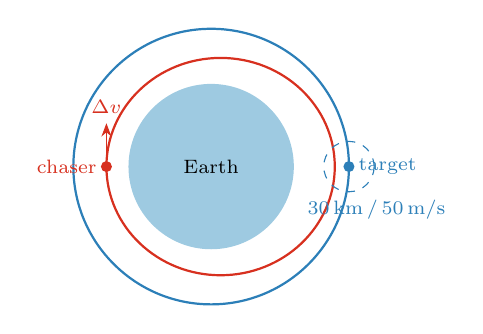
\begin{tikzpicture}[scale=1.0]
  \fill[earth] (0,0) circle (1.05); \node[font=\scriptsize] at (0,0) {Earth};
  \draw[blue2,thick] (0,0) circle (1.75);
  \draw[accent,thick] (0.12,0) ellipse (1.45 and 1.38);
  \fill[accent] (-1.33,0) circle (0.07) node[left,font=\scriptsize,accent] {chaser};
  \fill[blue2] (1.75,0) circle (0.07) node[right,font=\scriptsize,blue2] {target};
  \draw[blue2,dashed] (1.75,0) circle (0.32);
  \node[font=\scriptsize,blue2] at (2.1,-0.55) {\boxR\,/\,\boxV};
  \draw[-{Stealth},accent] (-1.33,0) -- ++(0,0.55) node[above,font=\scriptsize] {\dv};
\end{tikzpicture}
\end{column}
\begin{column}{0.55\textwidth}
\begin{itemize}\setlength{\itemsep}{2mm}
  \item \textbf{Success} \; inside \boxR\ and \boxV\ of the target
  \item \textbf{Failure} \; re-enter, escape, run dry, or run out of clock
  \item \textbf{Tank} \; 478\,m/s (15\,\% propellant); the generalist draws 353--656\,m/s per episode
  \item \textbf{Start} \; random orbits, phase gap up to $\pm180^\circ$; LEO 300--800\,km in the headline, up to 8,000\,km and $e\le0.3$ in the generalist
  \item \textbf{Act} \; a fixed-size burn, or a coast of 1\,min to 24\,h
\end{itemize}
\end{column}
\end{columns}
\note{Hooks: "how does fuel work" (rocket equation: 15 percent propellant at Isp 300 s is 478 m/s; bigger burns cost disproportionately more mass; the generalist sees its own tank size in the observation), "is that a lot" (a Hohmann 400 to 800 km is 217 m/s, so about 2x: enough for a good plan, not for random burning), "what is the phase gap" (angle along the orbit between chaser and target; the hard part of the task is closing it), "why those terminations" (every one is a real mission failure).}
\end{frame}

% ===================================================================== 2 loop
\begin{frame}{One loop, every decision}
\centering
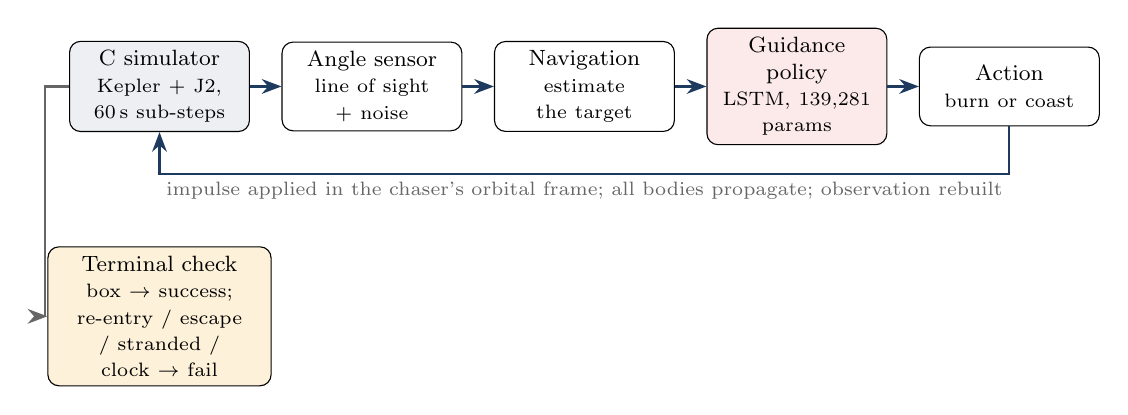
\begin{tikzpicture}[
  box/.style={draw,rounded corners,minimum height=1.0cm,text width=2.05cm,align=center,font=\footnotesize,fill=white},
  arr/.style={-{Stealth[length=2.5mm]},thick,navy}]
  \node[box,fill=navy!8] (sim) {C simulator\\{\scriptsize Kepler + J2, 60\,s sub-steps}};
  \node[box,right=0.4cm of sim] (sen) {Angle sensor\\{\scriptsize line of sight + noise}};
  \node[box,right=0.4cm of sen] (nav) {Navigation\\{\scriptsize estimate the target}};
  \node[box,right=0.4cm of nav,fill=accent!10] (pol) {Guidance policy\\{\scriptsize LSTM, \nParams\ params}};
  \node[box,right=0.4cm of pol] (act) {Action\\{\scriptsize burn or coast}};
  \draw[arr] (sim) -- (sen); \draw[arr] (sen) -- (nav); \draw[arr] (nav) -- (pol); \draw[arr] (pol) -- (act);
  \draw[arr] (act.south) |- ++(0,-0.6) -| (sim.south);
  \node[font=\scriptsize,grey] at ($(sim.south)!0.5!(act.south)+(0,-0.78)$) {impulse applied in the chaser's orbital frame; all bodies propagate; observation rebuilt};
  \node[box,below=1.45cm of sim,text width=2.6cm,fill=amber!15] (gate) {Terminal check\\{\scriptsize box $\to$ success; re-entry / escape / stranded / clock $\to$ fail}};
  \draw[arr,grey] (sim.west) -- ++(-0.3,0) |- (gate.west);
\end{tikzpicture}
\vspace{3mm}
\begin{itemize}\small
  \item The policy sees \nObs\ numbers and picks one of 31 actions. It never sees the target's true state in the angles-only configuration.
  \item The same loop runs in allocation-free C, action for action identical to PyTorch.
\end{itemize}
\note{Walk left to right. Hooks: "what are the 38 numbers" (appendix A1: own elements, fuel, estimated target, relative-motion block, the clock), "why an LSTM" (next slides), "what does the sensor give you" (direction only; one sentence from the briefing, then back to the policy).}
\end{frame}

% ===================================================================== 3 simulator
\begin{frame}{Simulator: analytic two-body plus J2, written in C}
\begin{columns}[c]
\begin{column}{0.4\textwidth}
\centering
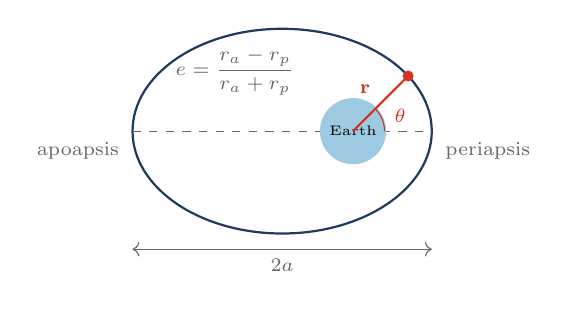
\begin{tikzpicture}[scale=1.0]
  \draw[navy,thick] (0,0) ellipse (1.9 and 1.3);
  \draw[grey,dashed] (-1.9,0) -- (1.9,0);
  \fill[earth] (0.9,0) circle (0.42); \node[font=\tiny] at (0.9,0) {Earth};
  \draw[grey,<->] (-1.9,-1.5) -- (1.9,-1.5) node[midway,below,font=\scriptsize] {$2a$};
  \fill[accent] (1.6,0.70) circle (0.07);
  \draw[accent,thick] (0.9,0) -- (1.6,0.70) node[midway,above left,font=\scriptsize] {$\mathbf r$};
  \draw[accent] (1.3,0) arc (0:45:0.4); \node[font=\scriptsize,accent] at (1.5,0.2) {$\theta$};
  \node[font=\scriptsize,grey,anchor=west] at (1.95,-0.25) {periapsis};
  \node[font=\scriptsize,grey,anchor=east] at (-1.95,-0.25) {apoapsis};
  \node[font=\scriptsize,grey] at (-0.6,0.75) {$e=\dfrac{r_a-r_p}{r_a+r_p}$};
\end{tikzpicture}
\end{column}
\begin{column}{0.6\textwidth}
\begin{itemize}\setlength{\itemsep}{1.5mm}
  \item \textbf{State} \; orbital elements $(a, e, i, \Omega, \omega, M)$
  \item \textbf{Propagate} \; Kepler's equation, closed form at any step
  \item \textbf{Burns} \; impulsive, fixed size
  \item \textbf{J2} \; Earth's bulge slowly rotates the orbit plane
\end{itemize}
\vspace{2mm}
\begin{block}{Why analytic}
Exact at any step size, so a 24-hour coast is one solve. About half a million environment steps per second on one laptop CPU.
\end{block}
\end{column}
\end{columns}
\note{Hooks: the elements picture (define a, e, theta from the sketch), "how do you solve Kepler" (Newton on E, then the half-angle formula to theta), "how did you validate it" (energy and angular momentum conserved; Hohmann 400 to 800 km matches 217 m/s; independent f and g oracle agreed to under a metre), "why J2" (the seventh skill uses nodal precession; A2).}
\end{frame}

% ===================================================================== 4 actions
\begin{frame}{Actions: a short menu of fixed burns and coasts}
\begin{columns}[c]
\begin{column}{0.46\textwidth}
\centering
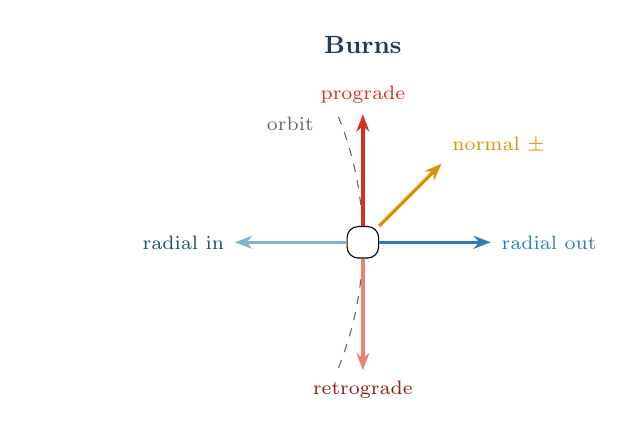
\begin{tikzpicture}[scale=1.25,arr/.style={-{Stealth[length=2.2mm]},very thick}]
  \node[font=\small\bfseries,navy] at (0,2.0) {Burns};
  \draw[grey,dashed] (-3.4,0) ++(-22:3.4) arc (-22:22:3.4);
  \node[font=\scriptsize,grey,anchor=east] at (-0.4,1.2) {orbit};
  \node[draw,fill=white,rounded corners,minimum size=0.4cm,inner sep=0] (c) at (0,0) {};
  \draw[arr,accent] (c) -- ++(0,1.3) node[above,font=\scriptsize,accent] {prograde};
  \draw[arr,accent!60] (c) -- ++(0,-1.3) node[below,font=\scriptsize,accent!60!black] {retrograde};
  \draw[arr,blue2] (c) -- ++(1.3,0) node[right,font=\scriptsize,blue2] {radial out};
  \draw[arr,blue2!60] (c) -- ++(-1.3,0) node[left,font=\scriptsize,blue2!60!black] {radial in};
  \draw[arr,amber!90!black] (c) -- ++(0.8,0.8) node[above right,font=\scriptsize,amber!90!black] {normal $\pm$};
\end{tikzpicture}
\end{column}
\begin{column}{0.54\textwidth}
\centering
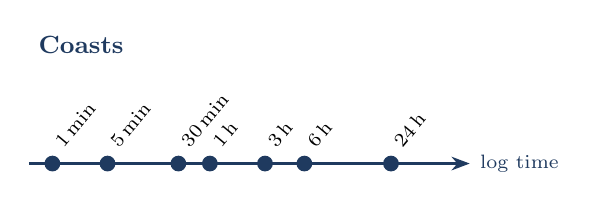
\begin{tikzpicture}[x=1cm]
  \node[font=\small\bfseries,navy,anchor=west] at (0,1.5) {Coasts};
  \draw[-{Stealth},thick,navy] (0,0) -- (5.6,0) node[right,font=\scriptsize] {log time};
  \foreach \x/\lab in {0.3/1\,min, 1.0/5\,min, 1.9/30\,min, 2.3/1\,h, 3.0/3\,h, 3.5/6\,h, 4.6/24\,h}{
    \fill[navy] (\x,0) circle (0.1); \node[font=\scriptsize,rotate=50,anchor=west] at (\x,0.15) {\lab}; }
\end{tikzpicture}
\end{column}
\end{columns}
\vspace{4mm}
\centering\small burn grades 1, 2, 5, 10, 25\,m/s \;$\cdot$\; 31 actions in all
\note{Hooks: "why not continuous thrust" (impulsive burns match chemical engines; a continuous head collapsed in early trials), "why do the long coasts matter" (credit assignment: without them the horizon is thousands of steps; with them the headline policy takes about 20 decisions per episode; physics and the sensor still run every 60 s inside a coast), "what frame are the burns in" (the chaser's own: along velocity, along the radius, along the orbit normal).}
\end{frame}

% ===================================================================== 5 policy
\begin{frame}{Policy and training}
\begin{columns}[c]
\begin{column}{0.48\textwidth}
\centering
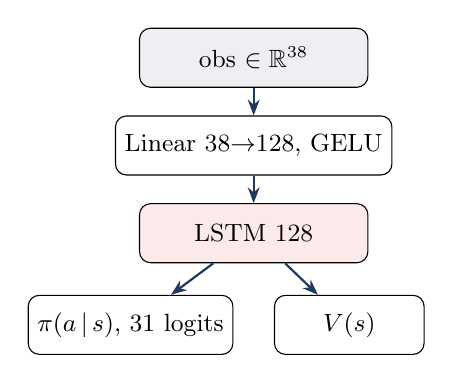
\begin{tikzpicture}[nb/.style={draw,rounded corners,minimum width=2.9cm,minimum height=0.75cm,font=\small,fill=white},arr/.style={-{Stealth[length=2mm]},thick,navy}]
  \node[nb,fill=navy!8] (o) {obs $\in\mathbb R^{\nObs}$};
  \node[nb,below=0.35cm of o] (e) {Linear \nObs$\to$128, GELU};
  \node[nb,below=0.35cm of e,fill=accent!10] (l) {LSTM 128};
  \node[nb,below left=0.4cm and -1.2cm of l,minimum width=1.9cm] (a) {$\pi(a\,|\,s)$, 31 logits};
  \node[nb,below right=0.4cm and -1.2cm of l,minimum width=1.9cm] (v) {$V(s)$};
  \draw[arr] (o)--(e); \draw[arr] (e)--(l); \draw[arr] (l)--(a); \draw[arr] (l)--(v);
\end{tikzpicture}
\end{column}
\begin{column}{0.52\textwidth}
\begin{itemize}\setlength{\itemsep}{2.5mm}
  \item \textbf{Small and recurrent} \; \nParams\ parameters; the LSTM carries what the last burn did
  \item \textbf{PPO} \; \nEnvs\ parallel environments, 50\,M steps per stage, about two hours each
  \item \textbf{Reward} \; $+1$ success, $-1$ failure, with potential-based shaping in between
  \item \textbf{Curriculum} \; one new difficulty per stage, warm-started
\end{itemize}
\end{column}
\end{columns}
\note{Hooks: "what is the shaping" (a potential on the mean-longitude gap and the orbit-shape mismatch; potential-based so it cannot change the optimal policy; the ablation without it peaks at 3.6 percent), "why PPO" (on-policy, stable with discrete actions, clipped ratio keeps updates small), "what is in the curriculum" (circular at full gap, then eccentric, wider altitudes, 3-D, estimate in the loop, then the seven-skill mixture; fresh training at the hard endpoint flat-lines), "why 1024 envs" (the simulator is cheap, so sample throughput is the lever).}
\end{frame}

% ===================================================================== 6 what it learned
\begin{frame}{What it learned, 2-D: phasing, shape matching, and when to wait}
\centering
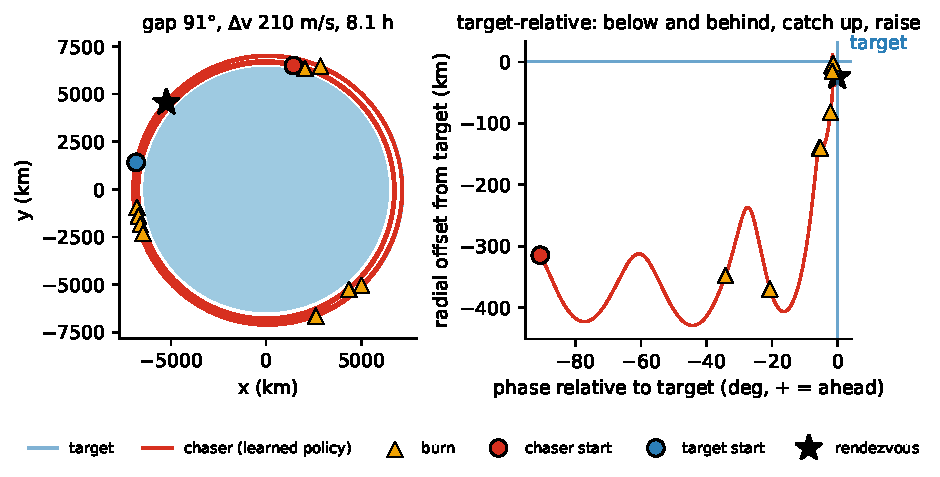
\includegraphics[width=0.66\textwidth]{traj_rendezvous.pdf}
\vspace{1mm}
\begin{itemize}\small
  \item \key{200/200} held-out episodes on \key{5/5 training seeds}; wide envelope (300--8,000\,km, $e\le0.30$) 800/800 on 4 seeds.
  \item Fuel: median 1.18$\times$ a two-impulse optimum on the same clock (appendix A4).
  \item Phasing by altitude, apse and eccentricity matching, and coasting through windows where a burn would not help.
\end{itemize}
\note{Point at the right panel: the chaser sits below and behind, the lower orbit's shorter period closes the gap, then it raises in steps. This is the textbook phasing manoeuvre; nobody told it. Hooks: "why does lower catch up" (T proportional to a^1.5; 100 km lower is about 4 degrees per orbit), "what is the comparator" (two-burn Lambert optimum, same episode, same clock; A5).}
\end{frame}

% ===================================================================== 7 generalist
\begin{frame}{One policy, seven rendezvous skills, in 3-D with J2}
\centering
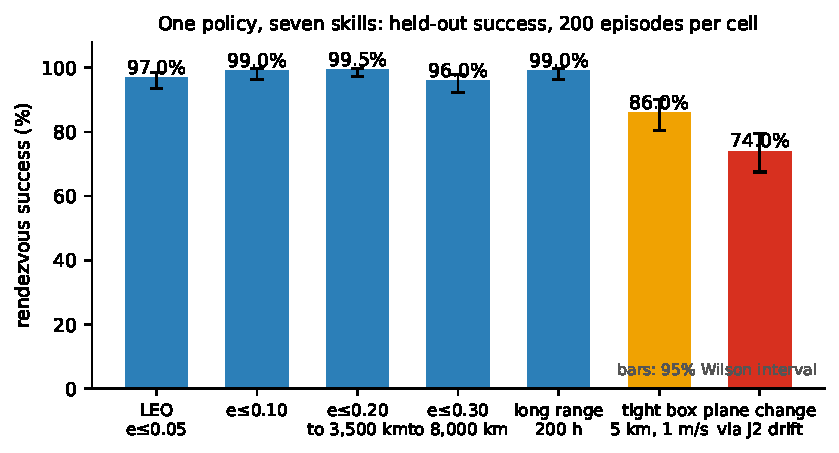
\includegraphics[width=0.8\textwidth,height=0.62\textheight,keepaspectratio]{generalist_cells.pdf}
\\[1mm]{\small Same network, same weights, every cell. 200 held-out episodes per skill, flying on the angles-only estimate.}
\note{Five skills at 96 to 99.5; the tight box at 86 (92.5 at its training fuel floor); the plane change at 74. Hooks: "what is the plane-change skill" (J2 nodal precession at a different altitude drifts the planes together; burning a 3 degree change would exceed the tank), "why one policy" (specialists score 6 to 42 percent off their home cell), "single seed?" (six of seven skills reproduce at a second seed; the seventh skill\'s final chain is one seed; A11).}
\end{frame}

% ===================================================================== 8 3-D episode
\begin{frame}{The same policy flying one 3-D episode}
\centering
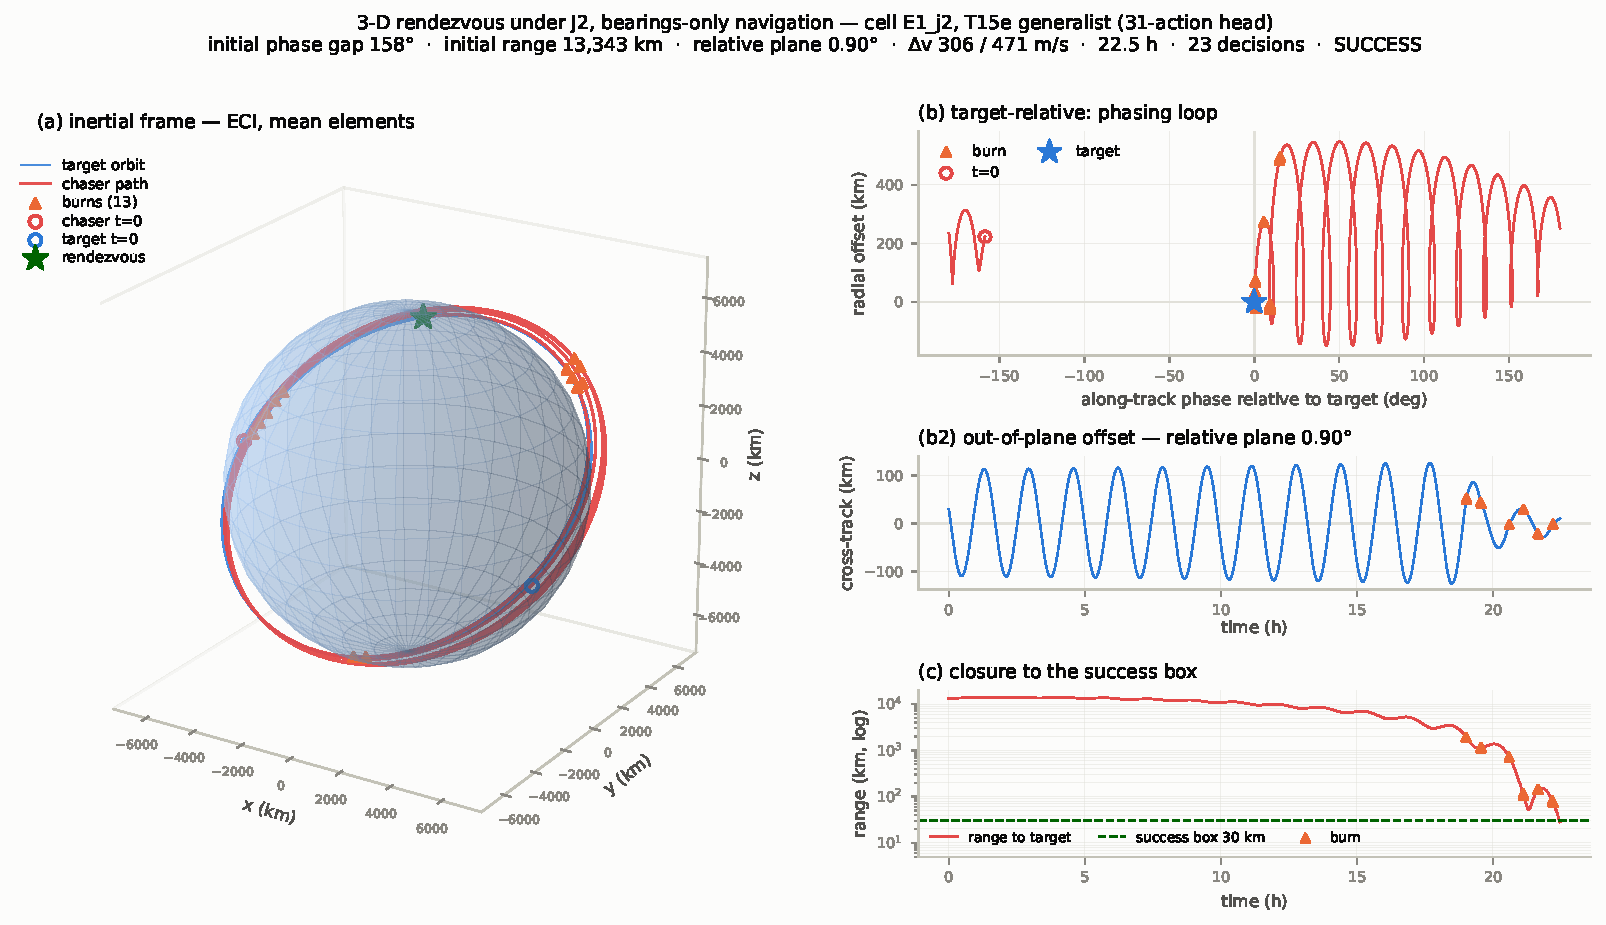
\includegraphics[width=0.92\textwidth,height=0.74\textheight,keepaspectratio]{traj3d_rendezvous.pdf}
\\[-1mm]{\scriptsize\textcolor{grey}{A $158^\circ$ gap and a $0.9^\circ$ plane difference closed in 22.5\,h with 306\,m/s and 23 decisions, on the filter's estimate of the target.}}
\note{Panel (b): parks above the target so the target catches up, then descends. Panel (b2): out-of-plane left alone until the end, then nulled with three normal burns. Panel (c): closure. Hook: "why wait on the plane" (plane burns are cheapest at the relative node and once, late).}
\end{frame}

% ===================================================================== 8b behaviour
\begin{frame}{What the policy actually does, scenario by scenario}
\centering
\IfFileExists{figs/generalist_behaviour.pdf}{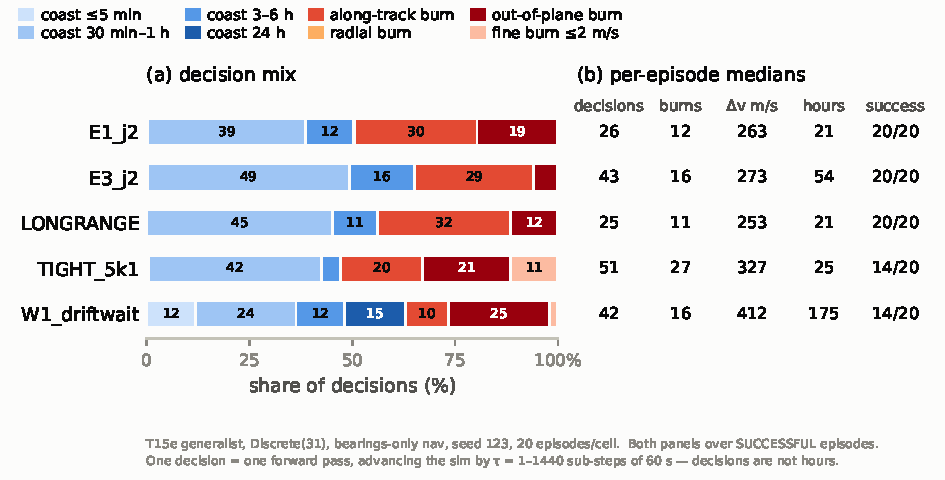
\includegraphics[width=0.9\textwidth]{generalist_behaviour.pdf}}{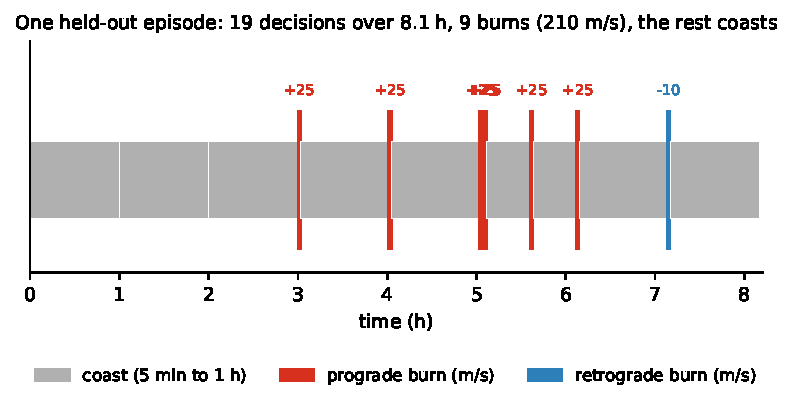
\includegraphics[width=0.8\textwidth]{decision_timeline.pdf}}
\\[1mm]{\scriptsize\textcolor{grey}{Decision mix of the seven-skill policy on five of its scenarios, 20 held-out episodes each (success rates on slide 8 are the 200-episode ones). The same weights coast a day at a time only when a plane gap can be drifted shut, use fine 1--2\,m/s burns only for the tight box, and never touch the radial burns.}}
\note{Hooks: "why so many coasts" (waiting is the cheapest manoeuvre), "why day-long coasts only on the plane-change cell" (J2 drift needs days; elsewhere they would waste the clock), "why fine burns on the tight box" (a 10 m/s quantum cannot land inside 1 m/s).}
\end{frame}

% ===================================================================== 9 close
\begin{frame}{What is open, and what I would do next}
\begin{columns}[T]
\begin{column}{0.5\textwidth}
\textbf{Open}
\begin{itemize}\setlength{\itemsep}{1.5mm}
  \item The seventh skill's final refinement chain is one training seed
  \item Fuel is 1.18$\times$ optimal; the burn grid is coarse
  \item Chaser navigation assumed perfect; no eclipses or sensor bias
\end{itemize}
\end{column}
\begin{column}{0.5\textwidth}
\textbf{Next}
\begin{itemize}\setlength{\itemsep}{1.5mm}
  \item Finer burn grades
  \item More seeds on the generalist
  \item A maneuvering target
\end{itemize}
\end{column}
\end{columns}
\note{Keep this short. Each open item is a hook you can answer: seeds (six of seven skills reproduce at a second seed; A11 has the table), fuel (coarse burn grid), chaser nav (common-mode error would need an augmented filter state). If asked what forces are modelled: point-mass gravity plus the secular J2 drift; no drag, no third body.}
\end{frame}

% ===================================================================== appendix
\appendix
\begin{frame}[plain]\centering{\Large\textcolor{navy}{\textbf{Appendix}}}\\[2mm]\small observation vector \;$\cdot$\; phasing and J2 \;$\cdot$\; the seven cells \;$\cdot$\; fuel audit \;$\cdot$\; Lambert search \;$\cdot$\; navigation \;$\cdot$\; C port \;$\cdot$\; the seventh skill \;$\cdot$\; FAQ \;$\cdot$\; verification \;$\cdot$\; seeds \;$\cdot$\; curriculum \;$\cdot$\; the seventh skill \;$\cdot$\; LSTM \;$\cdot$\; extensions \;$\cdot$\; PPO \;$\cdot$\; fuel awareness\end{frame}

\begin{frame}{A1 \; Observation vector (\nObs\ floats, roughly in $[-1,1]$)}
\tiny
\begin{tabular}{@{}lll@{}}
\toprule
slots & value & why\\
\midrule
0--1 & chaser altitude / scale, $e$ & size and shape\\
2--3 & $\sin\theta,\cos\theta$ & position on orbit, no wrap\\
4--5 & $v_r/v_{circ},\ v_t/v_{circ}$ & radial and tangential speed\\
6 & fuel fraction & budget remaining\\
7--8 & target altitude, $e$ (estimated) & target size and shape\\
9--12 & $\sin,\cos\,\omega$ for both & apse orientations\\
13--14 & $\sin,\cos\,\Delta\lambda$ (mean-longitude gap) & the phase gap\\
15 & (cap $-$ step)/cap & episode clock\\
16 & $\cos(\omega_s-\omega_t)$ & apsidal alignment\\
17--20 & nearest body: distance, bearing, closing rate, keep-out & Earth\\
21--25 & relative-inclination vector; $\Delta\mathbf e\cdot\hat h_t$; cross-track offset and rate & 3-D block\\
26--28 & $\dv_{plane},\ \dv_{remaining}$, feasibility margin & fuel ledger\\
29--30 & $\cos i_s,\ \cos i_t$ & J2\\
33--36 & LVLH radial / along-track offset; relative velocity, rotating-frame corrected & relative state\\
37 & target mean motion & \\
\bottomrule
\end{tabular}
\\[1mm]\textcolor{grey}{Target quantities are the filter's estimate in bearings-only mode. The policy is not given the covariance (tested: a $\sigma$ channel added nothing).}
\end{frame}

\begin{frame}{A2 \; Phasing, and plane change by burning versus by J2}
\small
\textbf{Phasing} \; $T = 2\pi\sqrt{a^3/\mu}$; a chaser 100\,km below a LEO target gains about $4^\circ$ of phase per orbit, so "drop, wait $N$ orbits, raise" is the textbook catch-up and it is what the policy does.\\[2mm]
\textbf{Plane change by burning} \; $\dv = 2v\sin(\Delta i/2)$. At 7.5\,km/s a $3^\circ$ change costs about 390\,m/s, most of a 478\,m/s tank.\\[2mm]
\textbf{Plane change by J2} \; Earth's equatorial bulge makes the node line drift around the pole at
\[ \dot\Omega = -\tfrac32\, J_2\, n \left(\frac{R_E}{p}\right)^{2} \cos i, \qquad p = a(1-e^2). \]
The rate depends on altitude and inclination, so two orbits at different altitudes drift apart in $\Omega$ at a controllable relative rate. Dip low, coast a day at a time, let the node drift close the plane gap, then raise. In the specialist about half of the plane alignment was bought this way.
\end{frame}

\begin{frame}{A3 \; The seven cells}
\scriptsize
\begin{tabular}{@{}lllllr@{}}
\toprule
cell & altitude band (km) & $e_{max}$ & box & clock (sub-steps) & success\\
\midrule
E0\_j2 & 300--800 & 0.05 & \boxR\,/\,\boxV & 3,000 & 97.0\,\%\\
E1\_j2 & 300--1,500 & 0.10 & \boxR\,/\,\boxV & 3,000 & 99.0\,\%\\
E2\_j2 & 300--3,500 & 0.20 & \boxR\,/\,\boxV & 4,500 & 99.5\,\%\\
E3\_j2 & 300--8,000 & 0.30 & \boxR\,/\,\boxV & 6,000 & 96.0\,\%\\
LONGRANGE & 300--3,500 & 0.12 & \boxR\,/\,\boxV & 12,000 & 99.0\,\%\\
TIGHT\_5k1 & 300--800 & 0.05 & 5\,km\,/\,1\,m/s & 3,000 & 86.0\,\%$^\dagger$\\
W1\_driftwait & 300--800 & 0.05 & \boxR\,/\,\boxV & 22,000 & 74.0\,\%\\
\bottomrule
\end{tabular}
\\[2mm]
$^\dagger$92.5\,\% at the training fuel floor. All cells: 3-D, J2 on, targets inclined $30$--$60^\circ$, relative plane up to $0.75$--$1^\circ$ ($2$--$5^\circ$ for W1), bearings-only navigation, Discrete(31) head, fuel budget sampled per episode (353--656\,m/s). Held-out seed 123, 200 episodes per cell, greedy actions, LSTM state zeroed per episode. A second training seed reproduces six of the seven cells (A11).
\end{frame}

\begin{frame}{A4 \; Fuel audit against a two-impulse optimum}
\begin{columns}[T]
\begin{column}{0.56\textwidth}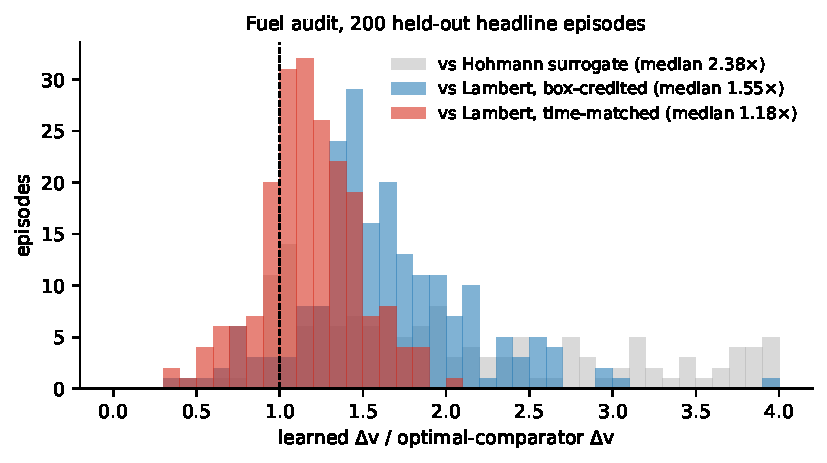
\includegraphics[width=\textwidth]{dv_ratio.pdf}\end{column}
\begin{column}{0.44\textwidth}\footnotesize
For each episode an offline solver finds the cheapest two-burn transfer from the chaser's start to the target, searching over how long to wait before the first burn and how long to fly, under the same clock the policy used.\\[1.5mm]
\textbf{Time-matched} \; must hit the target's exact position and velocity: median learned \dv\ is \key{1.18$\times$} it.\\[1mm]
\textbf{Box-credited} \; the same solution minus the 50\,m/s velocity tolerance the policy is never asked to close: \key{1.55$\times$}. The fairer of the two.\\[1.5mm]
{\scriptsize\textcolor{grey}{200 held-out episodes. Ratios below 1 happen because arrival is credited inside a box and a two-burn plan is not the unconstrained optimum.}}
\end{column}
\end{columns}
\end{frame}

\begin{frame}{A5 \; What the Lambert search looks like for one episode}
\begin{columns}[c]
\begin{column}{0.58\textwidth}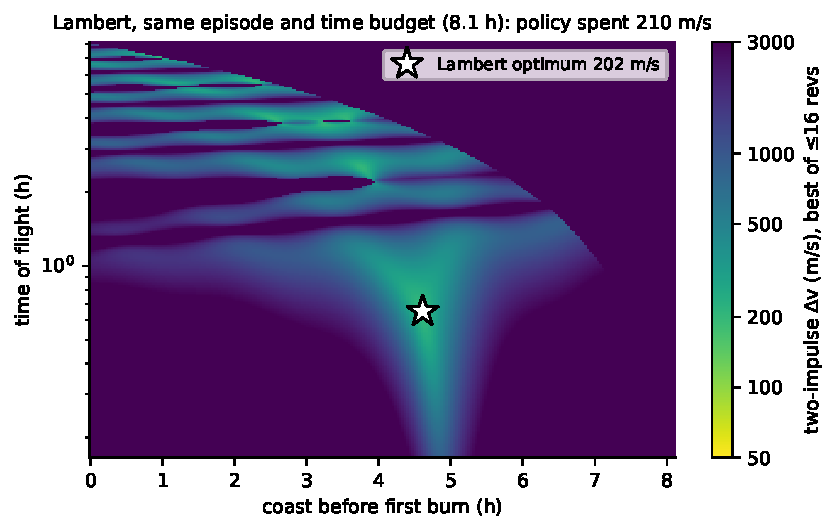
\includegraphics[width=\textwidth]{lambert_porkchop.pdf}\end{column}
\begin{column}{0.42\textwidth}\footnotesize
Every cell is one candidate plan: wait this long, then fly for that long. Colour is the two-burn \dv\ of the best conic connecting the two points in that time, including multi-revolution solutions. The banded structure is the orbital period showing through: cheap plans recur once per orbit.\\[1.5mm]
The star is the cheapest plan inside the policy's own clock. On this episode the optimum was 202\,m/s and the policy spent 210.
\end{column}
\end{columns}
\end{frame}

\begin{frame}{A6 \; Navigation in one picture: blind, acquire, converge}
\centering
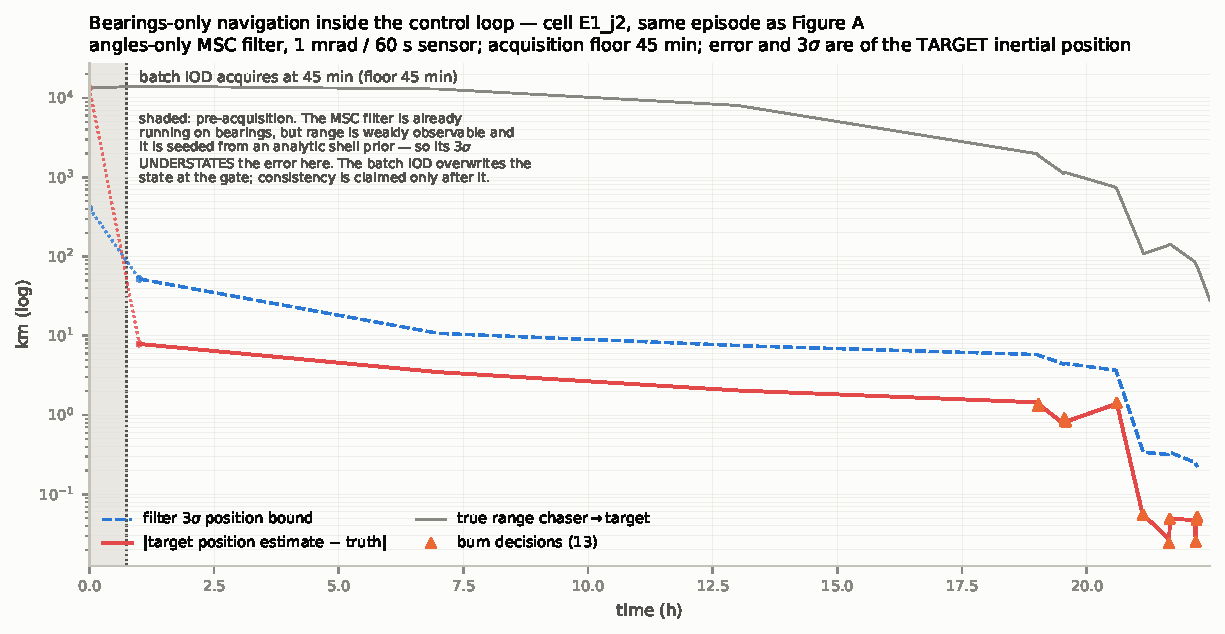
\includegraphics[width=0.72\textwidth]{nav3d_estimate.pdf}
\begin{columns}[T]
\begin{column}{0.5\textwidth}\scriptsize
The chaser measures only the direction to the target, not the distance. One direction tells you nothing about range; a sequence of directions while both orbits curve does. A batch solver tries many ranges along the first line of sight, propagates each, and keeps the one whose predicted directions match what was seen. That hands a full state to a recursive filter that keeps refining it.
\end{column}
\begin{column}{0.5\textwidth}\scriptsize
Policy result: trained on truth and handed the estimate, \key{51\,\%}; trained with the filter in the loop, \key{97\,\%} (2-D tight box) and \key{46$\to$98\,\%} across three seeds in 3-D. It learned to wait for acquisition and burn nothing while blind (median \dv\ before acquisition 75$\to$0\,m/s).
\end{column}
\end{columns}
\end{frame}

\begin{frame}{A7 \; C port of the policy}
\begin{columns}[T]
\begin{column}{0.5\textwidth}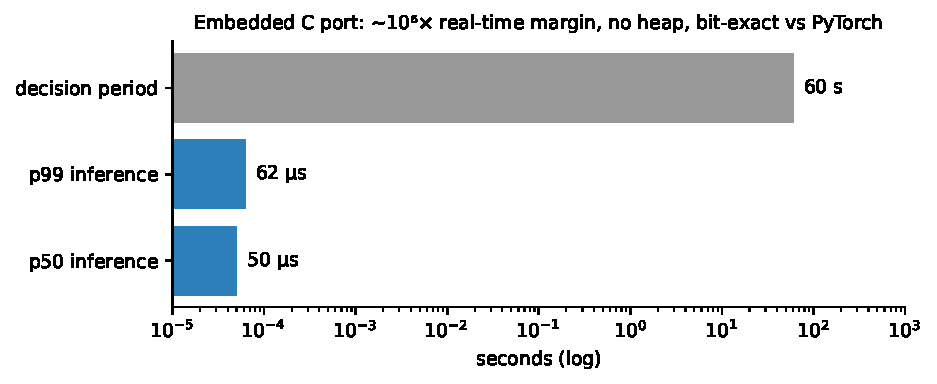
\includegraphics[width=0.95\textwidth]{cport_timing.pdf}\end{column}
\begin{column}{0.5\textwidth}\footnotesize
\begin{itemize}
  \item The trained weights exported to a C header; forward pass written by hand: linear, GELU, LSTM cell, two linear heads.
  \item No heap, no globals; the caller owns the 1\,kB of recurrent state; fixed work per call.
  \item Checked against PyTorch: identical action on 7,048 recorded observations and an identical action stream over 200 closed-loop episodes.
  \item Median 50\,$\mu$s per decision on a laptop against a 60\,s decision period (a benchmark, not a worst-case timing).
\end{itemize}
\end{column}
\end{columns}
\end{frame}

\begin{frame}{A8 \; How the seventh skill was trained}
\begin{columns}[T]
\begin{column}{0.5\textwidth}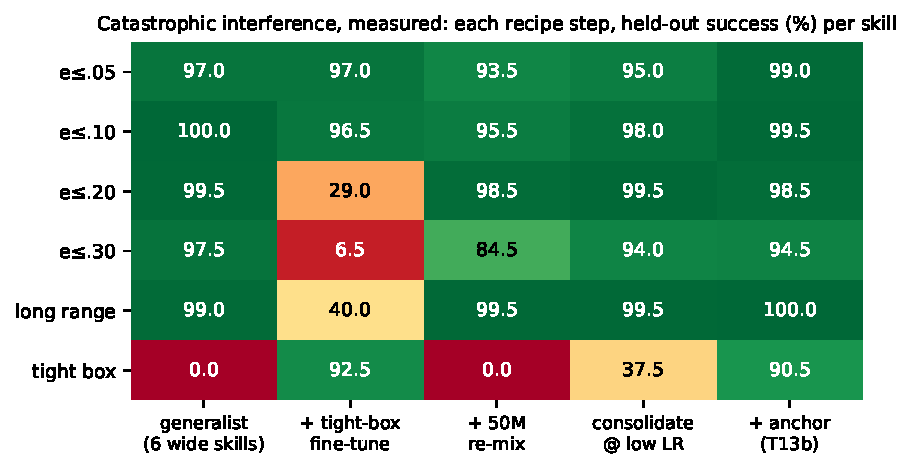
\includegraphics[width=\textwidth]{seesaw.pdf}\end{column}
\begin{column}{0.5\textwidth}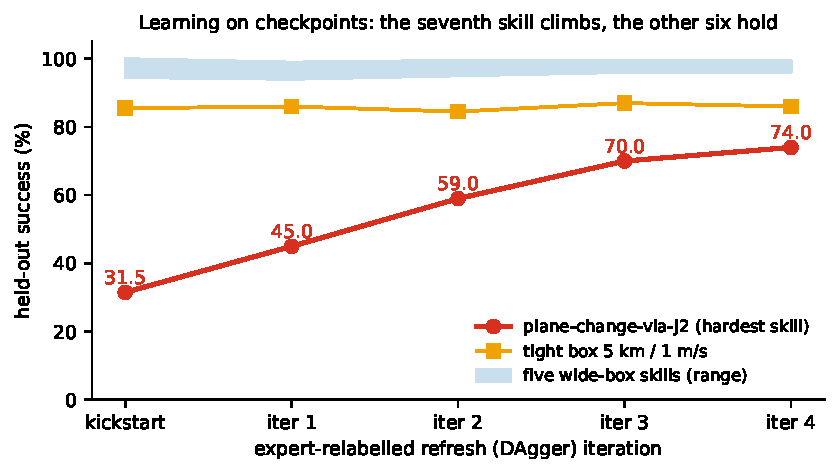
\includegraphics[width=\textwidth]{dagger_curve.pdf}\end{column}
\end{columns}
\small
\begin{itemize}
  \item Left: fine-tuning on one skill damaged others; a low learning rate plus replay of each skill's own trajectories held all six.
  \item Right: the plane-change skill never bootstrapped from reward. A scripted expert demonstrated it, the policy was refreshed on the expert's corrections four times, and each refresh was scored on 200 held-out episodes.
\end{itemize}
\end{frame}

\begin{frame}{A9 \; FAQ}
\scriptsize
\begin{description}
  \item[Why RL, when Lambert exists?] Lambert needs perfect state and gives an open-loop two-burn plan; the policy is closed-loop on an estimate, respects a budget, and one network covers seven regimes. Lambert is the grader, not the competitor.
  \item[Why discrete actions?] PPO is stable with them; a continuous head collapsed early on. The grid costs fuel (1.14--1.18$\times$ across two evaluation sets); finer grades are the obvious next step.
  \item[Is 200 episodes enough?] At 97\,\% the 95\,\% Wilson interval is about $\pm2.5$\,pp; for 0/200 failures the lower bound is 98.2\,\%. I report intervals, not "100\,\%".
  \item[Single seed?] The six-skill policy reproduced at a second training seed (tight box 92.5\,\%, wide cells 93.5--100\,\%). The seventh skill's four-step refinement was run once by design; its first two steps reproduced at a second seed with matching gains. The 2-D headline (5), wide envelope (4), 3-D nav and J2 rungs (3) are multi-seed.
  \item[Why coast 24\,h?] J2 nodal precession closes a plane gap for free; burning it would exceed the tank. The policy learned to wait.
  \item[How does the filter work?] Angles only, so range comes from how the bearing changes while the orbits curve; a batch solver picks the range that explains the first hour of bearings, then a recursive filter refines it. The finding I own is on the policy side: train on the estimate or lose 46 points.
  \item[What would you do differently?] Audit against physics from day one; log learning curves on every run; design the observation with the filter in mind from the start.
\end{description}
\end{frame}

\begin{frame}{A10 \; Verification measures}
\tiny
\begin{tabular}{@{}p{2.6cm}p{6.6cm}p{3.6cm}@{}}
\toprule
what & how & result\\
\midrule
Propagator & independent Lagrange $f$,$g$ oracle sharing no code; 980 adversarial episodes, 618k sub-steps & worst error 0.68\,m (float32 logging floor)\\
Conservation & energy and angular momentum on every coast step & at float precision\\
Transfer \dv & Hohmann 400$\to$800\,km and LEO$\to$GEO vs analytic & 217.02 vs 217.02\,m/s; 3856.7 vs 3856.7\\
Elements $\leftrightarrow$ Cartesian & 400 random round trips & median $3\times10^{-8}$\,m\\
Regression & three bitwise trajectory anchors (action-stream hash must not move) & caught real drift twice\\
Metrics & mutation test: 14 seeded errors in the evaluation code & 14/14 caught\\
Evaluation & held-out episode seed, greedy actions, Wilson intervals; 0/200 failures reported as $\ge98.2\,\%$ & every number on these slides\\
Comparator & two-impulse Lambert optimum per episode, same clock & 1.18$\times$ median\\
Filter & NEES / NIS in-bounds fractions (range/bearing EKF) & 94 / 95\,\%\\
C port & action agreement on 7,048 observations; 200 closed-loop episodes & 100\,\%; identical action stream\\
\bottomrule
\end{tabular}
\\[2mm]\textcolor{grey}{Sources: \texttt{T3\_RECOVERY\_CAMPAIGN.md} \S4--7, \texttt{PROGRESS.md} physics table, \texttt{scripts/orbital/embedded/results/}.}
\end{frame}

\begin{frame}{A11 \; Seeds and sample sizes}
\scriptsize
\begin{tabular}{@{}p{4.6cm}p{2.6cm}p{2.6cm}p{3.4cm}@{}}
\toprule
result & training seeds & held-out episodes & note\\
\midrule
2-D headline, 30\,km / 50\,m/s & 5 & 200 per seed (+500 at a second eval seed) & 200/200 every seed\\
2-D wide envelope (300--8,000\,km, $e\le0.30$) & 4 & 200 per seed & 800/800\\
3-D rendezvous, truth state & 3 & 200 per seed & 200/200 every seed\\
3-D bearings-only, tight box & 3 & 200 per seed & 589/600 pooled\\
J2 tight box, truth state & 3 & 200 per seed & 595/600 pooled\\
Six-skill generalist (anchored) & 2 & 200 per cell & seed 7: tight 92.5, wides 93.5--100\\
Seventh skill, refinement chain & 1 (steps 1--2 at a second seed) & 200 per cell & 74.0 at seed 42; 47.5 after two steps at seed 7\\
2-D policy-on-estimate, 51$\to$97 & 1 & 200 & replicated in 3-D across 3 seeds\\
\bottomrule
\end{tabular}
\\[2mm]\textcolor{grey}{Held-out means a fresh evaluation seed never used in training. 200 episodes at 97\,\% gives a 95\,\% Wilson interval of about $\pm2.4$ points.}
\end{frame}


\begin{frame}{A12 \; The curriculum: one new difficulty per stage, warm-started}
\scriptsize
\begin{tabular}{@{}llll@{}}
\toprule
stage & what changes & held-out result & cost\\
\midrule
L1 & circular orbits, full $\pm180^\circ$ phase gap, fresh weights & 200/200 & 50\,M steps ($\sim$2\,h)\\
L2 & eccentricity $\le0.05$, independent apse orientation & 200/200 & 50\,M\\
WL3, WL4 & altitude to 2,000 then 8,000\,km, $e$ to 0.30 & 200/200 each & 50\,M each\\
3-D & inclined planes, out-of-plane burns, 30-action head & 200/200 (3 seeds) & 50\,M\\
nav & filter estimate replaces truth in the observation & 97--98\,\% & 50\,M\\
J2 & secular drift on, tight box via three sub-rungs & 99.2\,\% (3 seeds) & 3 $\times$ 50\,M\\
mixture & seven cells sampled per episode, tank sampled & slide 8 & 50--200\,M\\
\bottomrule
\end{tabular}
\vspace{1mm}
\begin{itemize}\scriptsize
  \item \textbf{Why one variable per stage} \; fresh training at the hard endpoint flat-lined six times; each stage starts from a policy that already solves the previous one, so the new difficulty is the only thing left to learn.
  \item \textbf{How a stage was declared done} \; a pre-registered gate ($\ge60\,\%$ held-out, 3 seeds); in practice every rung cleared 200/200 before moving on.
  \item \textbf{Warm start}
\end{itemize}
\note{Two-minute answer. The order is "cheapest new information first": phasing is the core skill, so it is learned alone on circular orbits; shape, altitude, plane, estimate, drift are each added once the previous policy is at ceiling. Boundaries were set by what the previous policy failed on, measured, not by intuition. The 60 percent gate was the floor; nothing advanced below 100 percent in practice. Cost: 50M environment steps per rung is about two hours on a laptop CPU at half a million steps per second, so the whole chain is a day or two of compute.}
\end{frame}

\begin{frame}{A13 \; Why reward never found the seventh skill}
\begin{columns}[T]
\begin{column}{0.5\textwidth}\small
\textbf{The skill} \; close a $2$--$5^\circ$ plane gap by parking at a different altitude and letting J2 nodal precession drift the planes together over days, then rendezvous.\\[2mm]
\textbf{What reward offers} \; $+1$ at the end of a 175-hour episode, $-1$ otherwise, a shaping hint that cannot see the drift because it rewards closing the gap, not setting up the conditions that will close it later.\\[2mm]
\textbf{What exploration offers} \; a random policy must choose the day-long coast repeatedly, at the right altitude, with no intermediate signal. The probability is vanishing; 0/200 under every reward variant tried.
\end{column}
\begin{column}{0.5\textwidth}\small
\textbf{The fix} \; a scripted expert that knows the manoeuvre (91\,\% on the cell) demonstrates it; the policy is trained on those demonstrations (kickstart, 31.5\,\%), then refreshed four times on the expert's corrections of the states the policy itself visits (DAgger): 45, 59, 70, \key{74\,\%}.\\[2mm]
\textbf{Why DAgger and not plain imitation} \; a policy that only sees expert states drifts into states the expert never showed it and has no idea what to do; relabelling its own visited states closes that gap.\\[2mm]
\textbf{The framing} \; an exploration problem, not a capacity problem: the same 128-unit network holds the skill once shown it.
\end{column}
\end{columns}
\note{Stopping rule was written before the numbers: stop when a round closes less than 20 percent of the remaining gap to the teacher. Mechanism reproduced at a second seed: 33.5 kickstart, +14 on the first refresh, matching seed 42 step for step. The endpoint chain was run once by design.}
\end{frame}

\begin{frame}{A14 \; Why an LSTM, and what the memory carries}
\begin{columns}[T]
\begin{column}{0.52\textwidth}\small
\textbf{Partial observability} \; the policy sees the filter's estimate of the target, not the truth. Two things live only in history:
\begin{itemize}
  \item what the last burn did (the observation shows the state after, not the delta)
  \item where the filter is in its convergence (is the estimate still moving, or settled)
\end{itemize}
\vspace{1mm}
\textbf{Architecture} \; Linear 38$\to$128, GELU, LSTM 128, two linear heads. 139,281 parameters. Hidden and cell state (256 numbers) persist across decisions within an episode and are zeroed at reset.\\[1.5mm]
\textbf{Training detail} \; truncated backpropagation through time over 64 decisions; the recurrent state is carried across rollout boundaries.
\end{column}
\begin{column}{0.48\textwidth}\small
\textbf{The obvious alternative, tested} \; give the policy the filter's covariance directly ($\sigma$ of range over range) as an extra observation channel.\\[1mm]
\begin{tabular}{@{}lll@{}}
\toprule
arm & native & truth\\
\midrule
trained on estimate & 97.0\,\% & 97.0\,\%\\
same $+\sigma$ channel & 97.0\,\% & 98.5\,\%\\
\bottomrule
\end{tabular}
\\[1.5mm]
No change. The recurrent policy already infers what it needs about the estimate's quality from how the estimate moves.\\[1.5mm]
{\scriptsize\textcolor{grey}{200 episodes per arm, seed 123, 5\,km / 1\,m/s box. A memoryless control was never run; that ablation is on the list.}}
\end{column}
\end{columns}
\note{If asked "what does it remember": we did not probe the hidden state directly; the evidence is behavioural: the policy suppresses burns three-fold while the filter is blind and spends a median of zero before acquisition, which requires knowing acquisition has not happened, and that is not in the instantaneous observation. Honest gap: no feed-forward ablation.}
\end{frame}

\begin{frame}{A15 \; Extensions: a maneuvering target, and multiple agents}
\begin{columns}[T]
\begin{column}{0.5\textwidth}\footnotesize
\textbf{Maneuvering target} \; the navigation stack changes before the policy does.
\begin{itemize}
  \item today's filter assumes a ballistic target; an unmodelled burn shows up as a growing innovation and a diverging estimate
  \item first step: residual monitoring (a $\chi^2$ gate on the innovation) to detect a manoeuvre and inflate the covariance
  \item then an interacting-multiple-model filter: ballistic and manoeuvring hypotheses run in parallel, weighted by likelihood
  \item only then retrain the policy on the new estimate statistics, the same recipe as the 51$\to$97 step
\end{itemize}
\end{column}
\begin{column}{0.5\textwidth}\footnotesize
\textbf{Multiple agents} \; the shape I would build, not something I have built.
\begin{itemize}
  \item centralised training, decentralised execution: one critic sees every agent during training; each policy acts on its own observations at run time
  \item a communications model in the simulator (what each agent can see of the others, with delay and dropout), because the policy can only use what it would really have
  \item the simulator is already vectorised over 1,024 independent episodes; making agents share an episode is the structural change
\end{itemize}
{\scriptsize\textcolor{grey}{First reading: MAPPO (Yu et al.\ 2022); Bar-Shalom on IMM.}}
\end{column}
\end{columns}
\note{Do not bluff depth here. The honest line: "I have not built multi-agent; here is the structure I would start from and why the single-agent pieces carry over." The filter-first ordering for a maneuvering target is the defensible engineering point: a policy trained on a filter that cannot see manoeuvres will be confidently wrong.}
\end{frame}

\begin{frame}{A16 \; PPO details, as configured}
\footnotesize
\begin{columns}[T]
\begin{column}{0.46\textwidth}\scriptsize
\begin{tabular}{@{}lp{3.3cm}@{}}
\toprule
knob & value\\
\midrule
parallel environments & 1,024\\
steps per stage & 50\,M (mixture 200\,M)\\
discount $\gamma$ & 0.995\\
GAE $\lambda$ & 0.90\\
clip ratio & 0.2\\
entropy coefficient & 0.01\\
value loss weight & 2.0\\
epochs per batch & 1\\
minibatch & 8,192\\
BPTT horizon & 64 decisions\\
learning rate & 0.01 annealed; 0.001 consolidation\\
optimizer & Muon\\
reward clamp & $[-1,1]$ before GAE\\
\bottomrule
\end{tabular}
\end{column}
\begin{column}{0.54\textwidth}\footnotesize
\textbf{Reward} \; $+1$ success, $-1$ failure, $0$ at the clock cap. Dense term: potential-based shaping $\Phi(s')-\Phi(s)$ on the mean-longitude gap and the orbit-shape mismatch; with $\gamma_s=1$ it telescopes and cannot change the optimal policy.\\[1.5mm]
\textbf{Why these} \; $\gamma=0.995$ is a credit horizon of about 200 decisions; one epoch and a modest clip keep updates conservative with 1,024 correlated environments; entropy 0.01 kept the long coasts alive early (lower, and they died before the first success was sampled).\\[2mm]
{\scriptsize\textcolor{grey}{Never ablated: the 128 width, GELU, the LSTM itself. Library defaults, inherited rather than chosen.}}
\end{column}
\end{columns}
\end{frame}

\begin{frame}{A17 \; Fuel awareness: the same weights spend less when they have less}
\centering
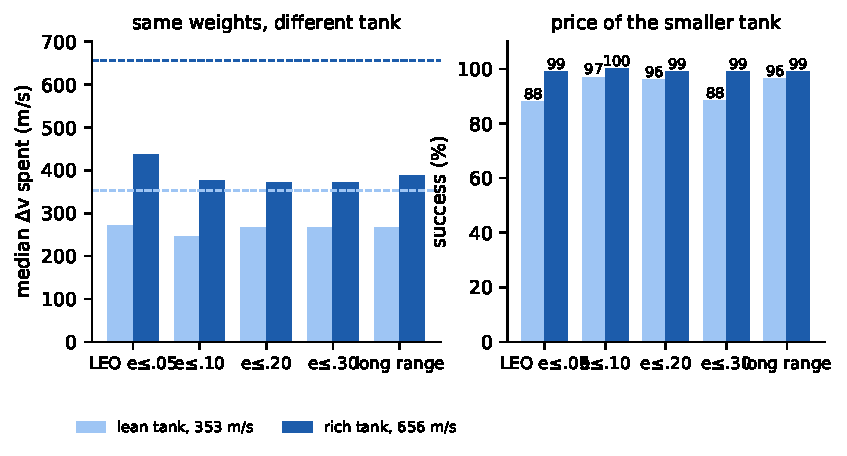
\includegraphics[width=0.7\textwidth]{fuel_aware.pdf}
\vspace{-1mm}
{\scriptsize Trained with the tank sampled per episode (353--656\,m/s) and shown its fuel fraction, the generalist spends about 40\,\% less on a lean tank than on a rich one, for 1 to 11 points of success.}
\end{frame}

\end{document}
